\chapter{Methodologies}

\label{chapter:methodologies}

In this chapter, we describe the methodologies used in this thesis.
Comprehensive source code reflecting these methodologies can be found in our
public GitHub
repository\footnote{https://github.com/atreyasha/spp-explainability}.

\section{Facebook Multilingual Task Oriented Dialog}

\citet{schuster-etal-2019-cross-lingual} originally released the Facebook
Multilingual Task Oriented Dialog (FMTOD) data set to encourage research in
cross-lingual transfer learning for Natural Language Understanding (NLU) tasks;
specifically from from high-resource to low-resource languages. The authors
released the FMTOD data set with English as the high-resource language providing
$\sim$43k annotated utterances, and Spanish and Thai as low-resource languages
providing a total of $\sim$14k utterances. Furthermore, they streamlined the
data set on two key tasks; namely intent detection and textual slot filling. In
this thesis, we focus solely on the English language intent detection task in
the FMTOD data set. This intent detection task entails a multi-label sequence
classification task with a total of 12 classes from alarm, reminder and
weather-related domains.

\subsection{Motivation}

We chose to work with the FMTOD data set since it is both a recently released
and well-studied data set
\citep{schuster-etal-2019-cross-lingual,zhang2019joint,zhang-etal-2020-intent}.
We focus on the English language intent classification task since it is a
relatively straightforward task which allows us to place a greater focus on
performance and explainability. Furthermore, the English language subset entails
the highest resources in the FMTOD data set. Finally, we find the FMTOD data
set's intent detection classification especially attractive because it allows us
to test the SoPa++ model on a multi-class NLU problem; which is significantly
different from the focus on binary classification sentiment detection tasks in
SoPa \citep{schwartz2018sopa}.

\subsection{Preprocessing}

We enumerate our preprocessing steps below:

\begin{enumerate}{}
  \item Similar to \citet{schwartz2018sopa}, we convert all FMTOD text samples
  to a lowercased format. This assists in simplifying the data set further.
  \item Next, we search through the pre-provided training, validation and test
  data partitions to remove duplicates within each partition.
  \item Finally, we remove data duplicates which overlap between partitions.
  During this step, we do not remove any cross-partition duplicates from the
  test partition in order to keep it as similar as possible to the original test
  partition. This comes into importance later when we compare performance
  evaluations on the test set with other studies.
\end{enumerate}

\begin{figure}[t]
  \centering
  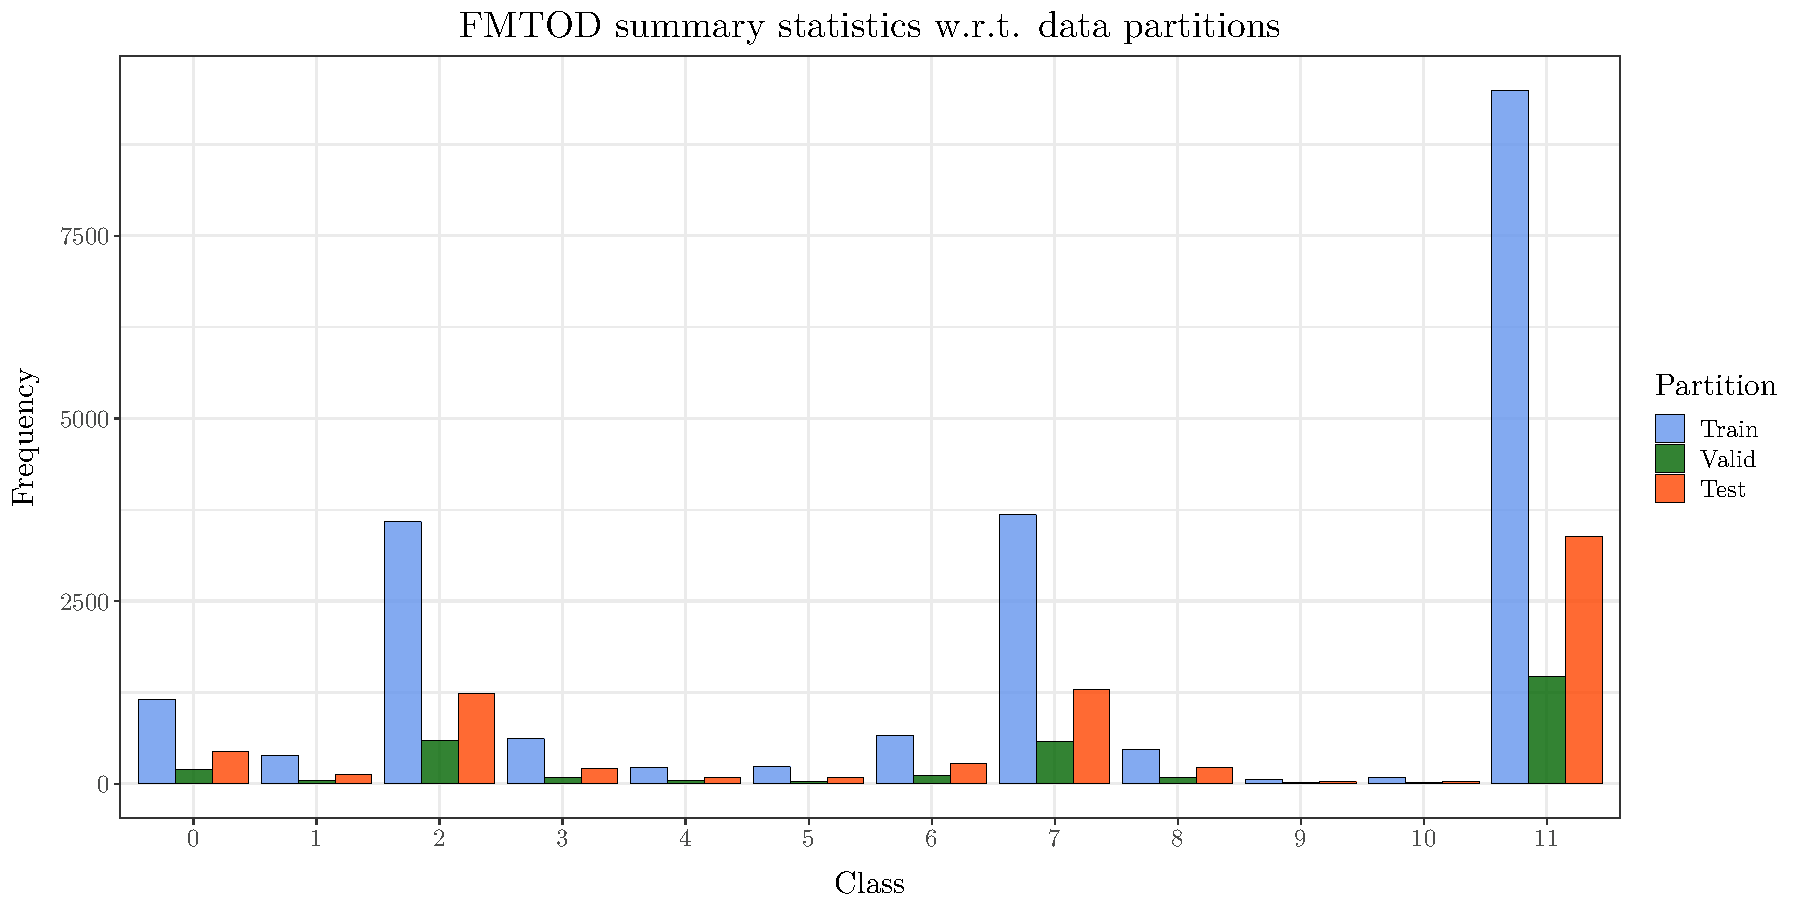
\includegraphics[width=14cm]{pdfs/generated/fmtod_summary_statistics.pdf}
  \caption{Data distribution of the preprocessed FMTOD data set grouped by
    classes and partitions}
  \label{fig:fmtod}
\end{figure}

\begin{table}[t!]
  \centering
  \begin{tabular}{lllll}
    \toprule
    Class and description & Train & Validation & Test & $\Sigma$ \\
    \midrule
    0: \texttt{alarm/cancel\_alarm} & 1157 & 190 & 444 & 1791 \\
    1: \texttt{alarm/modify\_alarm} & 393 & 51 & 122 & 566 \\
    2: \texttt{alarm/set\_alarm} & 3584 & 596 & 1236 & 5416 \\
    3: \texttt{alarm/show\_alarms} & 619 & 83 & 212 & 914 \\
    4: \texttt{alarm/snooze\_alarm} & 228 & 49 & 89 & 366 \\
    5: \texttt{alarm/time\_left\_on\_alarm} & 233 & 30 & 81 & 344 \\
    6: \texttt{reminder/cancel\_reminder} & 662 & 114 & 284 & 1060 \\
    7: \texttt{reminder/set\_reminder} & 3681 & 581 & 1287 & 5549 \\
    8: \texttt{reminder/show\_reminders} & 474 & 82 & 217 & 773 \\
    9: \texttt{weather/check\_sunrise} & 63 & 13 & 25 & 101 \\
    10: \texttt{weather/check\_sunset} & 88 & 11 & 37 & 136 \\
    11: \texttt{weather/find} & 9490 & 1462 & 3386 & 14338 \\[5pt]
    \hline \hline \\[-10pt]
    $\Sigma$ & 20672 & 3262 & 7420 & 31354 \\
    \bottomrule
  \end{tabular}
  \caption{Frequency of the preprocessed FMTOD data set classes grouped by
    partitions; $\Sigma$ signifies the cumulative frequency statistic}
  \label{tab:fmtod}
\end{table}

Many of the duplicates observed were already present in the original FMTOD data
set, with additional duplicates being created from the initial lowercasing step.
After preprocessing, we obtain a lowercased variant of the FMTOD data set with
strictly unique data partitions. In the next section, we describe the summary
statistics of the preprocessed FMTOD data set.

\begin{table}[t!]
  \centering
  \begin{threeparttable}
    \begin{tabular}{lll}
      \toprule
      Class and description & Utterance length$^{\dagger}$ & Example$^{\ddagger}$ \\
      \midrule
      0: \texttt{alarm/cancel\_alarm} & 5.6 $\pm$ 1.9 & cancel weekly alarm \\
      1: \texttt{alarm/modify\_alarm} & 7.1 $\pm$ 2.5 & change alarm time \\
      2: \texttt{alarm/set\_alarm} & 7.5 $\pm$ 2.5 & please set the new alarm \\
      3: \texttt{alarm/show\_alarms} & 6.9 $\pm$ 2.2 & check my alarms. \\
      4: \texttt{alarm/snooze\_alarm} & 6.1 $\pm$ 2.1 & pause alarm please \\
      5: \texttt{alarm/time\_left\_on\_alarm} & 8.6 $\pm$ 2.1  & minutes left on my alarm \\
      6: \texttt{reminder/cancel\_reminder} & 6.6 $\pm$ 2.2 & clear all reminders. \\
      7: \texttt{reminder/set\_reminder} & 8.9 $\pm$ 2.5 & birthday reminders \\
      8: \texttt{reminder/show\_reminders} & 6.8 $\pm$ 2.2 & list all reminders \\
      9: \texttt{weather/check\_sunrise} & 6.7 $\pm$ 1.7 & when is sunrise \\
      10: \texttt{weather/check\_sunset} & 6.7 $\pm$ 1.7 & when is dusk \\
      11: \texttt{weather/find} & 7.8 $\pm$ 2.3 & jacket needed? \\[5pt]
      \hline \hline \\[-10pt]
      $\mu$ & 7.7 $\pm$ 2.5 & \textemdash \\
      \bottomrule
    \end{tabular}
    \begin{tablenotes}[flushleft]
      \footnotesize
      \item $^{\dagger}$Summary statistics follow the mean $\pm$
      standard-deviation format
      \item $^{\ddagger}$Short and simple examples were chosen for brevity and
      formatting purposes
    \end{tablenotes}
  \end{threeparttable}
  \caption{Tabular summary of utterance length statistics and examples for FMTOD
    data classes; $\mu$ signifies the cumulative summary statistics}
  \label{tab:fmtod-examples}
\end{table}

\begin{table}[t!]
  \centering \def\arraystretch{1.3}
  \begin{tabular}{L{0.27\linewidth} L{0.45\linewidth} l}
    \toprule
    Study & Summary & Accuracy \\
    \midrule
    \citet{schuster-etal-2019-cross-lingual} & BiLSTM jointly trained on both the slot filling and intent detection English language tasks & 99.1$\%$ \\
    \citet{zhang2019joint} & BERT along with various decoders jointly fine-tuned on both the slot filling and intent detection English language tasks & 96.6--98.9$\%$ \\
    \citet{zhang-etal-2020-intent} & RoBERTa and XLM-RoBERTa fine-tuned on the English language and multilingual intent detection tasks respectively along with WikiHow pre-training & 99.3--99.5$\%$ \\
    \bottomrule
  \end{tabular}
  \caption{Tabular summary of studies that addressed the FMTOD intent detection
    English language task, along with their relevant summaries and accuracy
    range(s)}
  \label{tab:fmtod-results}
\end{table}

\subsection{Summary statistics}

Figure \ref{fig:fmtod} shows the summary statistics of the preprocessed FMTOD
data set grouped by classes and data set partitions. Similarly, Table
\ref{tab:fmtod} shows the same summary statistics in a tabular form with
explicit frequencies. Based on the summary statistics, we can observe that the
preprocessed FMTOD data set is significantly imbalanced with $\sim$45$\%$ of
samples falling into Class 11 alone. We take this observation into consideration
in later sections and apply fixes to mitigate this data imbalance. In addition,
we observe from Table \ref{tab:fmtod-examples} that input utterances in the
preprocessed FMTOD data set are generally short; with a mean input utterance
length of 7.7 and a standard deviation of 2.5 tokens. Utterance length summary
statistics were computed with the assistance of NLTK's default \texttt{Treebank}
word tokenizer \citep{bird-loper-2004-nltk}.

\subsection{Performance range}

Several studies have optimized deep learning models on the FMTOD English
language intent classification task using a variety of models from BiLSTMs to
XLM-RoBERTa
\citep{schuster-etal-2019-cross-lingual,zhang2019joint,zhang-etal-2020-intent}.
Table \ref{tab:fmtod-results} summarizes these studies along with their reported
accuracy scores on the FMTOD English language intent classification task. Based
on the presented results from these recent studies, we can infer that the
general competitive accuracy range for the FMTOD English language intent
classification task is from 96.6$\%$ to 99.5$\%$.

\section{SoPa++}

In this section we describe our SoPa++ model's architecture and present both
similarities and differences compared to the SoPa model in
\citet{schwartz2018sopa}.

\subsection{Tokenization and word embeddings}

Similar to \citet{schwartz2018sopa}, we utilize NLTK's default \texttt{Treebank} word
tokenizer \citep{bird-loper-2004-nltk} to conduct tokenization of input
utterances into word-level tokens. While \citet{schwartz2018sopa} utilize GloVe
840B 300-dimensional true-cased embeddings, we utilize GloVe 6B 300-dimensional
uncased word-level embeddings \citep{pennington2014glove} to project the input
tokens in utterances to continuous numerical spaces. We utilized this smaller
subset of word-level embeddings since it allowed us to work with lower-cased
words, as well as experiment with a variety of embedding dimensions during our
development phase.

\subsection{$\omega$-Weighted finite state automaton}

As mentioned in Section \ref{section:soft-patterns}, \citet{schwartz2018sopa}
constructed the SoPa model with an ensemble of linear-chain WFAs which permitted
both epsilon and self-loop transitions. As noted in Section
\ref{section:sopa-model-specs}, epsilon and self-loop transitions are useful
constructs in abstracting WFAs and allowing them to match variable length
strings. However based on our experimentation during our development phase, we
observed a key concern that the highest scoring paths in the WFAs in SoPa tended
to have a large variation of string lengths due to the effect of both
epsilon-transitions and self-loops. We believe that this reduced the impact
of SoPa's explainability methods and as a result, the first change we
decided for was to remove both epsilon and self-loop transitions. With this
change, we could at least ensure that each WFA would match strings of a fixed length.

However, matching strings of fixed lengths could also be seen as a form of overfitting in
the model; since a model could simply memorize short strings or phrases and
would not necessarily "learn" to generalize. To address this concern, we
decicded to include a new type of transition within the now strict linear-chain
WFAs; namely the wildcard transition which we define here as a
$\omega$-transition. Allowing for such a transition was only natural since
wildcards are already crucial parts of regular expressions; which as we
mentioned are equivalent to FAs. With this, we provide the following amended
definition for a $\omega$-WFA: 

\begin{definition}[$\omega$-Weighted finite-state automaton]
  \label{def:w-wsa}
  A $\omega$-weighted finite-state automaton over a semiring $\mathbb{K}$ is a 5-tuple
  $\mathcal{A} = \langle \Sigma, \mathcal{Q}, \Gamma, \lambda, \rho \rangle$,
  with:

  \begin{itemize}
    \itemsep0em
    \item[--] a finite input alphabet $\Sigma$;
    \item[--] a finite state set $\mathcal{Q}$;
    \item[--] transition weights $\Gamma: \mathcal{Q} \times \mathcal{Q} \times
    (\Sigma \cup \{\omega\}) \rightarrow \mathbb{K}$;
    \item[--] initial weights $\lambda: \mathcal{Q} \rightarrow \mathbb{K}$;
    \item[--] and final weights $\rho: \mathcal{Q} \rightarrow \mathbb{K}$.
  \end{itemize}

  \begin{remark}
    An $\omega$ transition is equivalent to a wildcard transition, which
    consumes an arbitrary token input and moves to the next state
  \end{remark}

  \begin{remark}
    Besides the inclusion of the $\omega$-transition and removal of the
    $\epsilon$-transition, an $\omega$-WFA has all of the same characteristics
    as the WFA defined in Definition \ref{def:wfa}.
  \end{remark}  
\end{definition}

With the removal of the epsilon and self-loop transitions, we were able to allow
for fixed string length matches to our WFAs. In addition, with the introduction
of the $\omega$-WFA, we are able to add a layer of generalization such that any
token input could possibly be accepted. Finally, similar to
\citet{schwartz2018sopa} we enforce that our $\omega$-WFAs all have a strict
linear-chain structure. They are now considered strict since we removed the
option of self-loop transitions.

%%% Local Variables: 
%%% mode: latex
%%% TeX-master: "main"
%%% End: 